\documentclass{article}
\usepackage{amsmath} % Required for mathematical symbols and fonts
\usepackage{graphicx} % Required for inserting images
\usepackage{tikz}

\usetikzlibrary{automata,positioning}

\usepackage{tikz-cd}
\usepackage{amssymb} % Required for additional mathematical symbols
\usepackage{amsthm}

\newcommand{\D}{
    \hat{\delta}_{D}
}

\newcommand{\N}{
    \hat{\delta}_{N}
}

\newcommand{\DD}[2]{
    \hat{\delta}_{D}(\{#1\}, #2)
}

\newcommand{\NN}[2]{
    \hat{\delta}_{N}(#1, #2)
}

\usetikzlibrary{automata}
\newtheorem{lemma}{Lemma}
\usepackage{mathtools}

\theoremstyle{remark}
\newtheorem*{remark}{Remark}
\usepackage[T1]{fontenc}
\usepackage{lmodern}

\title{Finite Automata Sheet}
\author{Gallo Tenis}
\begin{document}

\maketitle

\begin{center}
    \textit{
        Automata theory problems from the book ''Automata Theory, Languages, and Computation'' by J. Ullman.
    }
\end{center}
\section*{DFA and NFA equivalence}
\begin{enumerate}
    \item \textbf{(Equivalence theorem.)}
    If \( D = (Q_D, \Sigma, \delta_D, \{q_0\}, F_D) \) is the DFA constructed from NFA 
    \( N = (Q_N, \Sigma, \delta_N, q_0, F_N) \) by the subset construction, then \( L(D) = L(N) \).
    Conversely if $L$ is a language that is accepted by some DFA then it is accepted by some NFA.
    \\$\textbf{Proof.}$
    By definition of language of both $N$ and a generic DFA
    \[
    L(N) := \{w \in \Sigma^* : \hat{\delta}_N(q_0,w) \cap F_N \neq \varnothing\}
    \]
    \[
    L(D) := \{w \in \Sigma^* : \hat{\delta}_D(\{q_0\},w) \in F_D\}
    \]
    In our case, let $S = \DD{q_0}{w}$ (which is a state made of a set of $F_N$), then
    \[
    S \in F_D \iff S \cap F_N \neq \varnothing.
    \]
    In other words, the only thing to prove is that for any $w \in \Sigma^n$
    \[
        \DD{q_0}{w} = \NN{q_0}{w}.
    \]
    We need to rely in the transition function constructed by subsets out of $\N$.
    By induction on $n = \vert w \vert$:
    \begin{enumerate}
        \item[\textbf{Basis.}] Assume $n = 0$ so that $w = \varepsilon$. Then 
        the construction by subsets transition function will simply be $\delta_D(\{q_0\},\varepsilon) = \{q_0\}$ then 
        also we have
        \[
        \DD{q_0}{\varepsilon} = q_0 = \NN{q_0}{\varepsilon}.
        \]
        Thus we conclude that $\delta_D = \D = \N$ (under renaming the singleton set $\{q_0\}$ as $q_0$).
        \item[\textbf{Hypothesis.}] Assume that for the string $x$ of lenght $n$ it held that 
        \[
        \DD{q_0}{x} = \NN{q_0}{x} = \{p_1,\dots, p_m\} = S.
        \]
        \item[\textbf{Thesis.}] We have to prove that for a string $w = xa$ such that $n = \vert x\vert$ it follows that 
        \[
        \DD{q_0}{w} = \NN{q_0}{w}.
        \]
        To prove this assertion we recall the definition of $\D$ for any DFA and compare it to the one constructed by subsets.
        We have that 
        \begin{equation}
            \DD{q_0}{w} \stackrel{def}{=} \delta_D(\DD{q_0}{x},a)
        \end{equation}
        \begin{equation}
            \delta_D(S,a) \stackrel{c.b.s.}{=} \bigcup_{p \in S}\delta_N(p,a) = \bigcup_{i=1}^{m}\delta_N(p_i,a).
        \end{equation}
        Note that in (2), by construction $S$ is a subset of $Q_N$ such that
        \begin{equation}
            \DD{q_0}{w} = \delta_D(\DD{q_0}{x},a) = \delta_D(S,a)
        \end{equation}
        hence, the transition function constructed by subsets is a valid transition function for $D$.
        Furthermore by equation (1)
        \[
        \DD{q_0}{w} = \bigcup_{i=1}^{m}\delta_N(p_i,a).
        \]
        We also note that in the case of the extended transition function of $N$ 
        \[
        \NN{q_0}{w} \stackrel{def}{=} \bigcup_{i=1}^{m}\delta_N(p_i,a) = \delta_D(S,a) \stackrel{(3)}{=} \DD{q_0}{w}.
        \]
    \end{enumerate}
    Since 
    Conversely, to prove that a DFA $D = (Q_D, \Sigma, \delta_D, \{q_0\}, F_D)$ induced language is the same as some NFA language, 
    by structural induction on $n$, the lenght of the input string, we define the NFA $N$ as 
    \begin{enumerate}
        \item[\textbf{Basis.}]
        We let the start state $q_0$ of $D$ be the start state also of $N$. 
        So that for $w = \varepsilon$, $\DD{q_0}{\varepsilon} = \NN{q_0}{\varepsilon}$.
        \item[\textbf{Hypothesis.}]
        For $\vert x \vert = n$ suppose $\DD{q_0}{x} = p_n$ then we let $\NN{q_0}{x} = \{p_n\}$.
        \item[\textbf{Thesis.}]
        For $w = xa$ with $\vert w \vert = n+1$, by hypothesis 
        \[
        \DD{q_0}{w} = \delta_D(\DD{q_0}{x},a) = \delta_D(p_n,a) = p_{n+1}.
        \]
        We let $\NN{q_0}{w} = \{p_{n+1}\}$.
    \end{enumerate}
    \begin{flushright}
        \qed
    \end{flushright}

    \item \textbf{(Worst case.)} Show that there exists a NFA with $n$ states such that equivalent DFA  
    has $2^n$ states.\\
    $\textbf{Solution.}$
    We shall build an NFA that accepts univocally the language
    \[
    \{w\in \{0,1\}^*: \text{ the } n\text{-th} \text{ symbol from the end of } w \text{ is } 1\}.
    \]
    We first construct an NFA of this language having $n$ states.
    By structural induction on $\vert w \vert$
    \begin{enumerate}
        \item[\textbf{Basis.}]
        \item[\textbf{Hypothesis.}]
        \item[\textbf{Thesis.}]
    \end{enumerate}

    \item Prove that if \( N \) is an NFA that has at most one choice of state for any state and input symbol (i.e., \(\delta(q, a)\) never has size greater than 1), 
    then the DFA \( D \) constructed from \( N \) by the subset construction has exactly the states and transitions of \( N \) plus transitions to a new dead state whenever \( N \) is missing a transition
    for a given state and input symbol.\\
    $\textbf{Solution.}$
    Let $Q_N = q_0, q_1, \dots, q_n$.
    Consider the maximal case in which each state except possibly the last one has exactly one transition.
    Therefore the automaton is isomorphic to
    \begin{center} 
        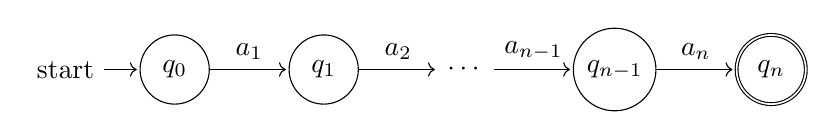
\begin{tikzpicture}[shorten >=1pt, node distance=1cm, auto]
            \node[state, initial](q_0) {$q_0$};
            \node[state](q_1)[right=of q_0] {$q_1$};
            \node(dots)[right=of q_1]{$\cdots$};
            \node[state](q_n-1)[right=of dots] {$q_{n-1}$};
            \node[state, accepting](q_n)[right=of q_n-1]{$q_n$};
            \path[->]
                (q_0) edge node {$a_1$}(q_1)
                (q_1) edge node {$a_2$}(dots)
                (dots) edge node {$a_{n-1}$}(q_n-1)
                (q_n-1) edge node {$a_{n}$}(q_n);
        \end{tikzpicture}
    \end{center}
    It is clear that the NFA described must accept only strings $w$ of lenght $n$.
    Else, for the sake of contradiction, suppose that the lenght were $k > n$ then, by pigeonhole principle
    there must exist at least one state $q_i$ such that for a symbol $a_i$; $\delta_{N}(q_{i},a_i) = \{p,r\}$, contradicting the fact 
    that $\delta_N(q,a)$ is a singleton (supposing that $k<n$ yields the same contradiction, but we get an unused state instead).

    We claim that $\NN{q_0}{w} = \{q_n\}$ this is, $\NN{q_0}{w}$ is a singleton.
    To prove this claim, by induction on $n$ the amount of states (not counting the starting one) and the lenght of the accepted strings
    \begin{enumerate}
        \item[\textbf{Basis.}] If $n = 1$, then by problem hypothesis
        \[
        \NN{q_0}{a_1} = \delta_N(q_0,a_1) = \{q_1\}.
        \]
        \item[\textbf{Hypothesis.}] Assume that for $n$ states and for a string $x = a_1\dots a_n$ we had 
        \[
        \NN{q_0}{x} = \{q_n\}.
        \]

        \item[\textbf{Thesis.}] We have to prove that for $n+1$ states and for a string $xa_{n+1}$ 
        \[
        \NN{q_0}{xa_{n+1}} = \{q_{n+1}\}.
        \]
        By hypothesis, 
        \[
        \NN{q_0}{xa_{n+1}} = \bigcup_{p \in \NN{q_0}{x}}\delta_N(p,a_{n+1}) = \bigcup_{p \in \{q_n\}}\delta_N(p,a_{n+1}) = \delta_N(q_n,a_{n+1})
        \]
        so by construction, 
        \[
        \delta_N(q_n,a_{n+1}) = \{q_{n+1}\}.
        \]
    \end{enumerate}

    By induction on $k$ the lenght of any accepted string (and the amount of states distincts from the starting one),
    we claim that the equivalent DFA yields the same states as the NFA plus a dead state.
    \begin{enumerate}
        \item[\textbf{Basis.}] For $k=2$ consider the transition table for the NFA,
        \[
            \begin{tabular}{c||c|c}
                & $a_1$ & $a_2$\\
                \hline\hline
                $\rightarrow$$q_0$ & $\{q_1\}$ & $\varnothing$\\
                $q_1$ & $\varnothing$ & $\{q_2\}$ \\
                $*q_2$ & $\varnothing$ & $\varnothing$  
            \end{tabular}
        \]
        Then, the transition table for the equivalent DFA will be 
        \[
            \begin{tabular}{c||c|c}
                & $a_1$ & $a_2$\\
                \hline\hline
                $\varnothing$ & $\varnothing$ & $\varnothing$\\
                $\rightarrow$$q_0$ & $\{q_1\}$ & $\varnothing$\\
                $q_1$ & $\varnothing$ & $\{q_2\}$ \\
                $*q_2$ & $\varnothing$ & $\varnothing$\\
                $\{q_0,q_1\}$ & $\{q_1\}$ & $\{q_2\}$\\
                $*\{q_0,q_2\}$ & $\{q_1\}$ & $\varnothing$\\
                $*\{q_1,q_2\}$ & $\varnothing$ & $\{q_2\}$\\
                $*\{q_0,q_1,q_2\}$ & $\{q_1\}$ & $\{q_2\}$
            \end{tabular}
        \]
        Changing names of states we see that 
        \[
            \begin{tabular}{c||c|c}
                & $a_1$ & $a_2$\\
                \hline\hline
                $\varnothing$ & $\varnothing$ & $\varnothing$\\
                $\rightarrow$$q_0$ & $\{q_1\}$ & $\varnothing$\\
                $q_1$ & $\varnothing$ & $\{q_2\}$ \\
                $*q_2$ & $\varnothing$ & $\varnothing$\\
                $A$ & $\{q_1\}$ & $\{q_2\}$\\
                $*B$ & $\{q_1\}$ & $\varnothing$\\
                $*C$ & $\varnothing$ & $\{q_2\}$\\
                $*D$ & $\{q_1\}$ & $\{q_2\}$
            \end{tabular}
        \]
        so that in particular, $A$ and $D$ are the same state, $B$ is the same state as $q_0$ and $C$ is the same state as $q_1$.
        Furthermore, we see that $A, D$ are unreachable. 
        We conclude that for $k = 2$ the transition table for the NFA is
        \[
            \begin{tabular}{c||c|c}
                & $a_1$ & $a_2$\\
                \hline\hline
                $\varnothing$ & $\varnothing$ & $\varnothing$\\
                $\rightarrow$$q_0$ & $\{q_1\}$ & $\varnothing$\\
                $q_1$ & $\varnothing$ & $\{q_2\}$ \\
                $*q_2$ & $\varnothing$ & $\varnothing$  
            \end{tabular}.
        \]

        \item[\textbf{Hypothesis.}]
        Assume that for a string $x = a_1\dots a_{k}$ of lenght $k$ it held that for an NFA $N$ with states $Q_N = \{q_0,\dots, q_k\}$ the equivalent DFA
        had same $k$ states as the NFA plus one dead state: $Q_D = \{q_0,\dots, q_k, \varnothing\}$.

        \item[\textbf{Thesis.}]
        Consider the string $a_1\dots a_k a_{k+1} = xa_{k+1}$, 
        this case can be seen by adding a column $a_{k+1}$, hence
        by the first claim,
        \[
        \NN{q_0}{xa_{k+1}} = \bigcup_{i=1}^{k}\delta_N(q_i,a_{k+1}) = \{q_{k+1}\}
        \]
        so that the DFA also transitions to the singleton $\{q_{k+1}\}$ only in the state $q_k$ by subset construction.
        Then, necessarily $q_{k+1}$ transitions to $\varnothing$ since there are not further states.

        We see that by hypothesis all the subsets of $\{q_0,\dots,q_k\}$
        that are not singletons are unreachable, then since the only 
        reachable state starting from $q_{k}$ is $q_{k+1}$ and $q_{k+1}$ transitions to $\varnothing$,
        it follows that any subset state of $\{q_1,\dots, q_{k},q_{k+1}\}$ is unreachable.
    \end{enumerate}
    \begin{flushright}
        \qed
    \end{flushright}
\end{enumerate}
\section*{$\varepsilon$-NFA}

\section*{Regular expressions}
\end{document}